\section{Code Generation}
Nearing the end, of the compiler, after doing all the contextual analysis, you end up with a decorated syntax tree which has made sure that everything lives up to the programming language that has got defined earlier in this report. Then it is time for code generation.
Here there can be multiple code generators, as it can follow the visitor pattern to generate the code. This is the point where the designer of the compiler decides what the resulting language of the compiler should be. Whether it should be C, Assembly, or other programming languages depends on what the programming language is intended for and what machines the targeted language compiler should be able to run on. 
A good approach for high level languages is to translate to a intermediate low level language that already have implementations for most hardware.  
In that way instead of making many compilers for each high level language to target hardware from D => B, E => B, D => C, E => C, you can create one compiler from the high-level language to the intermediate language. If you want to output to multiple low-level languages, you need to add another compiler from the intermediate language to the new low-level language. In that way, instead of making a high-level \* low-level number of compilers, make High-level \+ Low-level number of compilers. It adds abstraction but might also add complexity if either the source language or the destination language has structures that are hard or impossible to implement. Some examples of compilers with intermediate languages are Java and C\#. Java compiles Java Bytecode which is the instruction set of the Java Virtual Machine. C\# compiles to Common Intermediate Language, which is then run on the Common Language Runtime.\\
\\
Taken a look into the code generation. There are 3 code generator visitors in total. The first one being C Code Generator, which is generating C code from the AST visitor. The second one is Arduino C code generator, which has the special features from the Arduino library, for example serial.print and many more. The last one is Java Bytecode generator for Jasmin. As there is a lot of code in these generators, and visitors has been explained in the previous chapter, we will focus on the code generation part from each of these code generator visitors.
The first code snippet is from the C code generator visitor, which are using its start node to include the necessary C headers within the generated code : \\
\begin{figure}[H]
\centering
\frame{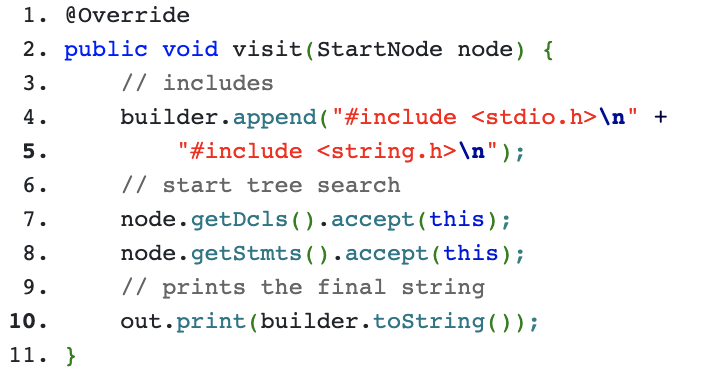
\includegraphics[scale=0.70]{figures/ew/io01.png}}
\label{io01}
\end{figure}
The second case, is where we have the Arduino C code generator.
\begin{figure}[H]
\centering
\frame{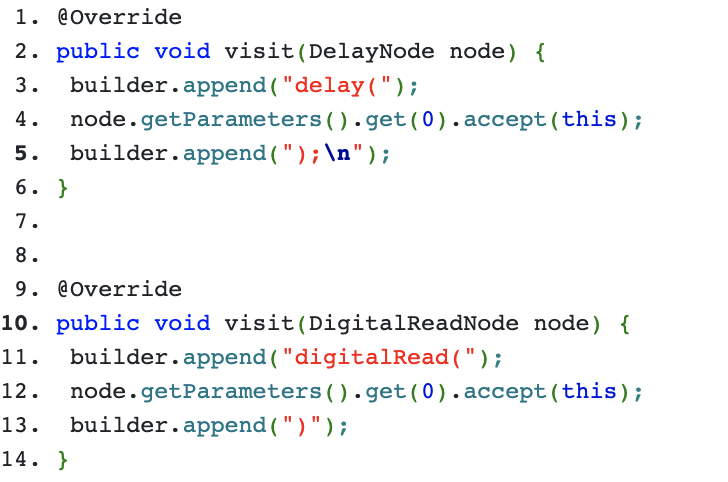
\includegraphics[scale=0.70]{figures/ew/io02.png}}
\label{io02}
\end{figure}
In example on figure \ref{io02}, we got two visitor function, both the delay node and the digital read node. Each of these will append the special Arduino library functions to the code generator, if it read the function id as both within the buildastvisitor. \\
\\
The last visitor is the Jasmin code generator.\\
Unlike the previous two visitors, the jasmin code generator doesn't compile to a C-like language, but rather to Jasmin, which is an assembler-representation of Java bytecode. This is quite different from parsing to C or Java, as the scoping rules are a bit different, either being completely flat inside a given function, or more of a nested structure if one is using classes and access modifiers. This combined with a register-based storage model means, that the compiler has to manually keep track of the allocated registers, and when it is safe to overwrite a given register with another value. This is currently handled when the Jasmin visitor visits a block node in the AST. The code snippet in question can be seen in listing \ref{code:JasminBlock}. Note that a copy of the variable environment is reset to its pre-block state after the entire block has been generated. This is so that a variable declared in an inner scope will take precedence when being referenced in an expression, compared to a variable of the same name declared previously in an outer scope, while still "deallocating" the inner variables after the block has been processed.
\begin{lstlisting}[caption={Code for visiting a block in the JasminCodeGeneratorVisitor}, label={code:JasminBlock}]
$$@Override
public void visit(BlockNode node) {
    List<String> oldVariableEnvironment = new ArrayList<String>(currentVariableEnvironment);
    List<String> oldLocalFunctions = new ArrayList<String>(currentLocalFunctions);
    // < Code for visiting children omitted for readability>
    currentVariableEnvironment = oldVariableEnvironment;
    currentLocalFunctions = oldLocalFunctions;
}
\end{lstlisting}

Furthermore, it should be considered that the JVM is a stack machine, and thus it should be taken into consideration, when writing code for it. Though this is mostly a fact to be considered when evaluating expressions, though it is also important when it comes to function calls (or method invocations, as they are parsed down to), as these use the top i elements of the stack as parameters, and then push the return value of the function back on the stack. The stack also plays a role in some of the more complex implementations (namely prints and strings), as these use object references like in Java, but on the stack, like any other value. It isn't terribly hard to write the (java) method invocations, but you do have to keep your wits about you, as the order of the stack matters, and the typing syntax of the JVM gets a bit longer and incomprehensible, when referencing custom types like "String".
